\subsection{Architecture}

The building blocks of any convolutional neural network are convolution layers,
which, as stated previously, are small-sized learnable filters that are
convolved across an input tensor, and output a visual stimulus under the form of
another tensor, then fed into the next layer.

\begin{figure}[h]
	\center
	\resizebox{480pt}{!}{
		\begin{tikzpicture}
\tikzstyle{connection}=[ultra thick,every node/.style={sloped,allow upside down},draw=\edgecolor,opacity=0.7]
%%%%%%%%%%%%%%%%%%%%%%%%%%%%%%%%%%%%%%%%%%%%%%%%%%%%%%%%%%%%%%%%%%%%%%%%%%%%%%%%%%%%%%%%
%% Draw Layer Blocks
%%%%%%%%%%%%%%%%%%%%%%%%%%%%%%%%%%%%%%%%%%%%%%%%%%%%%%%%%%%%%%%%%%%%%%%%%%%%%%%%%%%%%%%%
% conv1_1,conv1_2
\pic[shift={(0,0,0)}] at (0,0,0) {RightBandedBox={name=cr1,caption=conv1,%
        xlabel={{"64","64"}},ylabel=224,zlabel=224,fill=\ConvColor,bandfill=\ConvReluColor,%
        height=40,width={2,2},depth=40}};
%pool1
\pic[shift={(0,0,0)}] at (cr1-east) {Box={name=p1,%
        fill=\PoolColor,opacity=0.5,height=35,width=1,depth=35}};
%%%%%%%%%%
% conv2_1,conv2_2
\pic[shift={(2,0,0)}] at (p1-east) {RightBandedBox={name=cr2,caption=conv2,%
        xlabel={{"64","64"}},zlabel=112,fill=\ConvColor,bandfill=\ConvReluColor,%
        height=35,width={3,3},depth=35}};
%pool2
\pic[shift={(0,0,0)}] at (cr2-east) {Box={name=p2,%
        fill=\PoolColor,opacity=0.5,height=30,width=1,depth=30}};
%%%%%%%%%%
% conv3_1,conv3_2
\pic[shift={(2,0,0)}] at (p2-east) {RightBandedBox={name=cr3,caption=conv3,%
        xlabel={{"256","256","256"}},zlabel=56,fill=\ConvColor,bandfill=\ConvReluColor,%
        height=30,width={4,4,4},depth=30}};
%pool3
\pic[shift={(0,0,0)}] at (cr3-east) {Box={name=p3,%
        fill=\PoolColor,opacity=0.5,height=23,width=1,depth=23}};
%%%%%%%%%%
% conv4_1,conv4_2,conv4_3
\pic[shift={(1.8,0,0)}] at (p3-east) {RightBandedBox={name=cr4,caption=conv4,%
        xlabel={{"512","512","512"}},zlabel=28,fill=\ConvColor,bandfill=\ConvReluColor,%
        height=23,width={7,7,7},depth=23}};
%pool4
\pic[shift={(0,0,0)}] at (cr4-east) {Box={name=p4,%
        fill=\PoolColor,opacity=0.5,height=15,width=1,depth=15}};
%%%%%%%%%%
% conv5_1,conv5_2,conv5_3
\pic[shift={(1.5,0,0)}] at (p4-east) {RightBandedBox={name=cr5,caption=conv5,%
        xlabel={{"512","512","512"}},zlabel=14,fill=\ConvColor,bandfill=\ConvReluColor,%
        height=15,width={7,7,7},depth=15}};
%pool5
\pic[shift={(0,0,0)}] at (cr5-east) {Box={name=p5,%
        fill=\PoolColor,opacity=0.5,height=10,width=1,depth=10}};
%%%%%%%%%%
% fc6
\pic[shift={(3,0,0)}] at (p5-east) {RightBandedBox={name=fc6,caption=fc6,%
        xlabel={{"1",""}},zlabel=4096,fill=\FcColor,bandfill=\FcReluColor,%
        height=3,width=3,depth=100}};
%%%%%%%%%%
% fc7
\pic[shift={(2,0,0)}] at (fc6-east) {RightBandedBox={name=fc7,caption=fc7,%
        xlabel={{"1","dummy"}},zlabel=4096,fill=\FcColor,bandfill=\FcReluColor,%
        height=3,width=3,depth=100}};
%%%%%%%%%%
% fc8
\pic[shift={(1.5,0,0)}] at (fc7-east) {RightBandedBox={name=fc8,caption=fc8+softmax,%
        xlabel={{"1","dummy"}},fill=\FcColor,bandfill=\FcReluColor,%
        height=3,width=3,depth=25}};

%%%%%%%%%%
% softmax
\pic[shift={(0,0,0)}] at (fc8-east) {Box={name=softmax,%
        xlabel={{"","dummy"}},zlabel=K,opacity=0.8,fill=\SoftmaxColor,%
        height=3,width=1.5,depth=25}};
    
%%%%%%%%%%%%%%%%%%%%%%%%%%%%%%%%%%%%%%%%%%%%%%%%%%%%%%%%%%%%%%%%%%%%%%%%%%%%%%%%%%%%%%%%
%% Draw Arrow Connections
%%%%%%%%%%%%%%%%%%%%%%%%%%%%%%%%%%%%%%%%%%%%%%%%%%%%%%%%%%%%%%%%%%%%%%%%%%%%%%%%%%%%%%%%
\draw [connection]  (p1-east)        -- node {\midarrow} (cr2-west);
\draw [connection]  (p2-east)        -- node {\midarrow} (cr3-west);
\draw [connection]  (p3-east)        -- node {\midarrow} (cr4-west);
\draw [connection]  (p4-east)        -- node {\midarrow} (cr5-west);
\draw [connection]  (p5-east)        -- node {\midarrow} (fc6-west);
\draw [connection]  (fc6-east)       -- node {\midarrow} (fc7-west);
\draw [connection]  (fc7-east)       -- node {\midarrow} (fc8-west);
\draw [connection]  (softmax-east)   -- node {\midarrow} ++(1.5,0,0);
%%%%%%%%%%%%%%%%%%%%%%%%%%%%%%%%%%%%%%%%%%%%%%%%%%%%%%%%%%%%%%%%%%%%%%%%%%%%%%%%%%%%%%%%
%% Draw Dotted Edges 
%%%%%%%%%%%%%%%%%%%%%%%%%%%%%%%%%%%%%%%%%%%%%%%%%%%%%%%%%%%%%%%%%%%%%%%%%%%%%%%%%%%%%%%%
\draw[densely dashed]
    (fc6-west)++(0, 1.5*.2, 1.5*.2) coordinate(a) -- (p5-nearnortheast)
    (fc6-west)++(0,-1.5*.2, 1.5*.2) coordinate(b) -- (p5-nearsoutheast)
    (fc6-west)++(0,-1.5*.2,-1.5*.2) coordinate(c) -- (p5-farsoutheast)
    (fc6-west)++(0, 1.5*.2,-1.5*.2) coordinate(d) -- (p5-farnortheast)
    
    (a)--(b)--(c)--(d)
    ;
%%%%%%%%%%%%%%%%%%%%%%%%%%%%%%%%%%%%%%%%%%%%%%%%%%%%%%%%%%%%%%%%%%%%%%%%%%%%%%%%%%%%%%%%
\end{tikzpicture}

	}
	\caption{The famous VGG-16 topology.}
	\label{fig:vgg16}
\end{figure}

	\subsubsection{Typical inputs and outputs}
In a typical CNN, input and output layers are of a fixed size corresponding to
the problem formulation. The input tensor representing an image can be of any
dimensions, usually with the shape $(H, W, C)$ for $H$ rows corresponding to the
image's height, $W$ columns for its width, and of third axis size $C$ for its
channels (usually 1 for grayscale images and 3 for RGB images). However, this
common input shape is not a restriction, and it usually depends on the approach
to the problem: it might be wiser to use square images of cropped grayscale
portraits for face recognition, for instance.\\

\todo{Add tikz image for input and output tensors/vectors}

As for the output, the shape is entirely dependent on the problem and the
desired output of the network. In common image classification implementations,
a one-hot (or multi-hot) encoded vector is usually used as ground truth label,
meaning that the expected output of the network is a vector of size $N$ for $N$
classes.

\begin{wrapfigure}{r}{0.4\textwidth}
	\begin{center}
		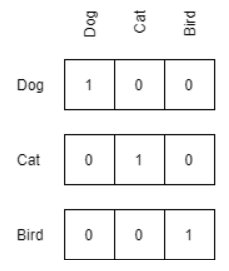
\includegraphics[width=0.24\textwidth]{figure/one_hot.png}
	\end{center}
	\label{fig:onehot}
	\caption{One-hot encoding of 3 classes. [temp, will make my own]}
\end{wrapfigure}


A one-hot encoded vector is a simple representation of the class to which a
given image belongs, where every value is either 0 for the indices
corresponding to the classes which the image does not belong to, or 1 otherwise
(see figure~\ref{fig:onehot}).\\

Nevertheless, there are many other possible output formats for convolutional
neural networks, such as another image for the case of auto-encoders or image
segmentation networks. One strong limitation of CNNs is their fixed-sized
input and output layers, which enforces them to be fed with strictly
constrained data. To bypass this constraint, another kind of neural network
must be used, such as recurrent neural networks.

	\subsubsection{Layer types}

The peculiarities of convolutional neural networks are mainly in the typical
kinds of layers that were not seen in the original perceptron. As it can be seen
on figure~\ref{fig:vgg16}, convolution layers are usually put in sequence, each
being smaller than the preceding, as to filter images in a coarse to fine
fashion.\\

The convolution layer owns its naming to the convolution operator, which
consists of summing up the element-wise multiplication between two matrices. In
the case of a CNN, the input layer -- either the input image, or an activation
map produced by a convolution layer -- is convolved with a relatively small
feature detection matrix, called a kernel or filter. The former is learnt by the
network during the training phase, and can be very different from layer to
layer, providing different features detection such as edges, contours, curves,
colors, shapes \emph{etc}\ldots

The kernel is slid over the convolved tensor by $N$ pixels (usually 1), called
the stride, and this dot-product is then appended to the output tensor named
the activation map, or feature map.

What results is a reduced tensor containing the relevant features in the image,
which preserves the spatial relationship between pixels. Having more convolution
layers, and thus more kernels or feature detectors, obviously results in more
features being extracted from the image, and therefore yielding more information
to be used in the final stage of the network, which can make the model more
accurate and more generalized.

Note that convolution layers can also be used in a hasty master, to achieve
deconvolution as to upsample an input and generate a higher-resolution tensor.
This practice can be seen in the auto-encoder model, where the goal is to
reconstruct an image from little information of an input.

\todo{Insert convolution picture here}
\begin{figure}[h]
	\center
	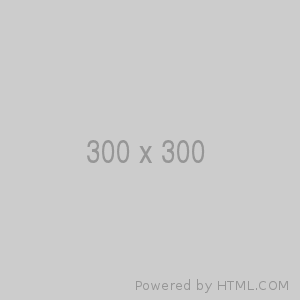
\includegraphics[width=0.4\textwidth]{figure/300x300.png}
	\label{fig:convolution}
	\caption{Convolution of a tensor by a kernel.}
\end{figure}


~\\It is very common to see pooling or sub-sampling layers in-between two
successive convolution layers. The role of the former is to reduce the
dimensionality of the feature map, while preserving the relevant information.

As it can be observed on figure~\ref{fig:pooling}, the choice between maximum
pooling and average pooling can have a great impact on the performance of a
network, depending on the input data and the overall configuration of the
layers. 
\newpage

\begin{figure}[h]
	\centering
	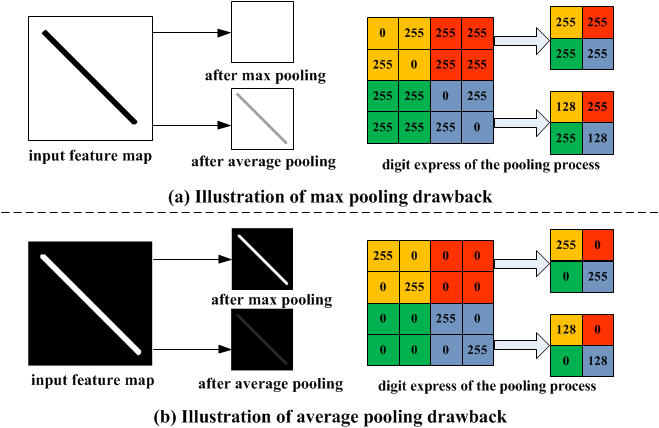
\includegraphics[width=0.8\textwidth]{figure/max_vs_avrg_pooling.png}
	\label{fig:pooling}
	\caption{Max pooling VS average pooling. [temp, will make my own]}
\end{figure}

The work of Yu \etal~\cite{MixedPooling} introduces a novel pooling
technique that is supposed to overcome this problem while also addressing the
overfitting issue, by randomly choosing between max and average pooling
methods.\\

Last but not least, a very important aspect of neural networks is their
natural tendency to produce linear classifiers at each layer. This can be
explained by how each layer computes its outputs, as in the following naive
single-layer perceptron (\ref{linear_perceptron}):

\begin{equation} \label{linear_perceptron}
	f(o_i) = \displaystyle\sum_{j=0}^{N} w_{ij}x_j+\beta_0
\end{equation}


where $o_i$ is the $i^{th}$ output neuron, $N$ is the number of input neurons,
$w_{ij}$ is the weight, $x_j$ is the input neuron and $\beta_0$ is the bias for
the layer. This simple perceptron does not have the ability to classify
non-linear data, as it can clearly be seen by its linear equation, and
therefore does have a very limited interest.

In order to introduce linearity, an activation function is added to the
equation, as such:

\begin{equation} \label{nonlinear_perceptron}
	f(o_i) = \phi(\displaystyle\sum_{j=0}^{N} w_{ij}x_j+\beta_0)
\end{equation}

There exist different activation functions, such as the commonly used ReLU (for
Rectified Linear Units) defined as:

\begin{equation} \label{relu}
	f(x) = max(0, x)
\end{equation}

The reason why ReLU and its variants are so widely used in the state-of-the-art
neural networks over others such as Sigmoid or TanH, is mainly for its
efficient computation (both for the forward pass and the back-propagation), and
its sparse activation in randomly initialized networks.

\begin{figure}[h]
	\centering
	\begin{tikzpicture}
		\pgfplotsset{
			axis lines=middle,
			grid style={dotted,gray,line width=.1pt}
		}

		\begin{axis}[
			xlabel={x},
			ylabel={y},
			extra x ticks=0,
			x label style={at={(current axis.right of origin)},anchor=north west,below=1mm},
			y label style={at={(current axis.above origin)},anchor=south east},
			grid=both]
			\addplot+[domain=-5:4.5,samples=100,thick,mark=none,blue] {(x>=0)*x};
		\end{axis}
	\end{tikzpicture}
	\caption{The ReLU activation function.}
\end{figure}

By adding non-linear activation functions at the output of every layer in a
network, it is able to classify non-linearly separable datasets, which
represents most real world case studies in machine learning.\\


\subsubsection{Deep residual networks}

Nevertheless, other types of layers have seen the light thanks to the extensive
research in the field, and the classic structure of \emph{convolution, pooling,
activation, fully connected} is being surpassed by more sophisticated
architectures like \emph{deep residual networks} which outperform most
convolutional neural networks in the field of image recognition.\\

Originally introduced by He \etal~\cite{He_2016_CVPR}, deep residual networks
provide a way of constructing very deep convolutional neural networks, while
leveraging the power of residual blocks to greatly reduce the number of
parameters.

Indeed, the intuition of famous models such as AlexNet or VGG-16--which
achieved state-of-the-art classification at the time they were released--is to
make deeper and deeper networks to increase the accuracy of the convolution
filters.

However, it has been observed that simply stacking up layers presents a severe
issue: the gradients are \emph{vanishing or exploding} during the
back-propagation of the error. This can be explained by the way gradients are
computed and propagated backwards to every layer: since they are calculated by
the chain rule, and in the case of activation functions squeezing the outputs
in the $[0,1]$ range, the gradients arriving at the top layers of a network end
up being too small to have any impact on the learning of the corresponding
filters, thus the appellation ``vanishing'' gradients. On the other hand,
``exploding'' gradients are the result of the back-propagation of gradients
with an activation function that can produce larger values, such as ReLU.\\

The idea introduced with residual networks, is to pass information from
higher-level layers in the hierarchy to layers further down, as to provide
additional information on the input. In truth, the deeper layers of a CNN can
lack of context over their given activation map, and by preserving information
across the network, results have shown that it not only performs better, but
as Veit \etal~\cite{ResnetBehavior} have pointed out, the performance of the
network is more evenly spread across its layers than regular networks like
VGG-16, where removing one layer can cause a drastic decrease in accuracy.

\begin{figure}[h]
	\centering
	\begin{tikzpicture}[node distance=1.5cm,-latex]

		\node[draw, rectangle,minimum width=1cm,minimum height=0.5cm] (layer1) {weight layer};
		\node[draw, rectangle,minimum width=1cm,minimum height=0.5cm,below of=layer1] (layer2) {weight layer};
		\node[draw,circle,below of=layer2] (sum) {\Large$+$};

		\draw ($(layer1.north)+(0,1cm)$) -- (layer1) node[anchor=east,midway] {$\mathbf{x}$};
		\draw (layer1) -- (layer2) node[anchor=east,midway] {relu};
		\draw (layer2) -- (sum) node[anchor=east,midway] {relu};
		\draw ($(layer1.north)+(0,0.5cm)$) -- ++(1.5cm,0) |- (sum) node[pos=0.25,anchor=west] {$\mathbf{x}$};
		\draw (sum) -- ++(0,-1.2cm) node[midway,anchor=east] {relu};
		\node[anchor=north] (f2) at ($(sum)+(0,-1.2cm)$) {$\mathcal{F}(\mathbf{x}) + \mathbf{x}$};

		\draw [-,decorate,decoration={brace,amplitude=10pt}]
			($(layer2.south west)+(-0.1cm,0)$) -- ($(layer1.north west)+(-0.1cm,0)$) node [black,midway,anchor=east,xshift=-0.3cm]  {$\mathcal{F}(\mathbf{x})$};

	\end{tikzpicture}
	\label{fig:resblock}
	\caption{The building block of deep residual learning.}
\end{figure}

More precisely, every block of stacked layers is made to fit a residual
mapping, instead of the desired underlying mapping, expressed as:

\begin{equation}
	\mathcal{F}(x):=\mathcal{H}(x)-x
\end{equation}

where $\mathcal{H}(x)$ is the desired function to be fit, and $x$ is the output of a
higher-level block. By adding $x$ to the residual mapping $\mathcal{F}(x)$ via a shortcut
connection, the block of layers is indirectly made fitting the original
function $\mathcal{H}(x)$.

The hypothesis made in this paper is that this residual
mapping is easier for the network to fit onto than the original one, since it
only needs to minimize the residual (or the prediction error), rather than to
approximate the identity mapping.
